\setcounter{chapter}{1}
\chapter{Neuroanatomy}
\label{chap:neuro}
%
% \cleanchapterquote{We are part of the universe that has developed a remarkable ability: We can hold an image of the world in our minds. We are matter contemplating itself.}{Sean Carroll}{The Particle at the End of the Universe}
%
%
\paragraph{TODO}
\begin{itemize}
    \item was für parameter treten wo im Gehirn auf
\end{itemize}
%
%
\section{Introduction}
%
Neuroanatomy is the study of the structure of the brain.
Its task is to study the sizes, regions and structure of the nervous system in humans and animals.
This is quite a difficult task because the brain, especially the human brain, is one of the most complex organs with a great diversity of cells, connections, topography and resulting functionalities.
Recently, techniques such as \ac{dMRI}, fluorescence microscopy, stained microscopy, autoradiography (to name a few), have been able to study more and more structures from different angles in the brain with different resolutions, modalities and contrasts on different species.
Different species help to understand the evolution of the brain. The brains of rodents and monkeys are not as large or as evolved as the human brain, but are still close in evolutionary terms.
\par
%
This chapter gives a general overview of the structure of the brain with its most important structures.
The main focus is on the nerve fiber architecture, since this is the focus of this work.
Additionally information can be found \eg{} \dummy{}.
%
%
%
\section{Brain Architecture}
%
The human brain (see \cref{fig:humanBrain}) consists of three main parts: the cerebellum, located at the rear bottom, the cerebrum, located at the top, and the brainstem.
The brainstem is the connection between the different brain areas and the spinal cord.
It can be further subdivided into the midbrain, the pons and the medulla obiongata, which in turn are further specialized.
The most important function of the cerebellum in the human brain is motor control.
It is highly folded and thus has a particularly large surface area, which will be important in a later stage.
\par
%
The cerebrum in the human brain is the largest part.
It is also folded and has a left and right hemisphere.
In addition, the cerebrum can be divided into 4 visible parts, which are separated by commissures (\eg{} sulcus centralis):
%
\begin{figure}[!t]
\centering
% \hspace*{\fill}
\subcaptionbox{\label{fig:brainLobes}Side view human brain. Frontal lobe,  Origin: \url{https://en.wikipedia.org/wiki/Frontal_lobe}}[.47\textwidth]{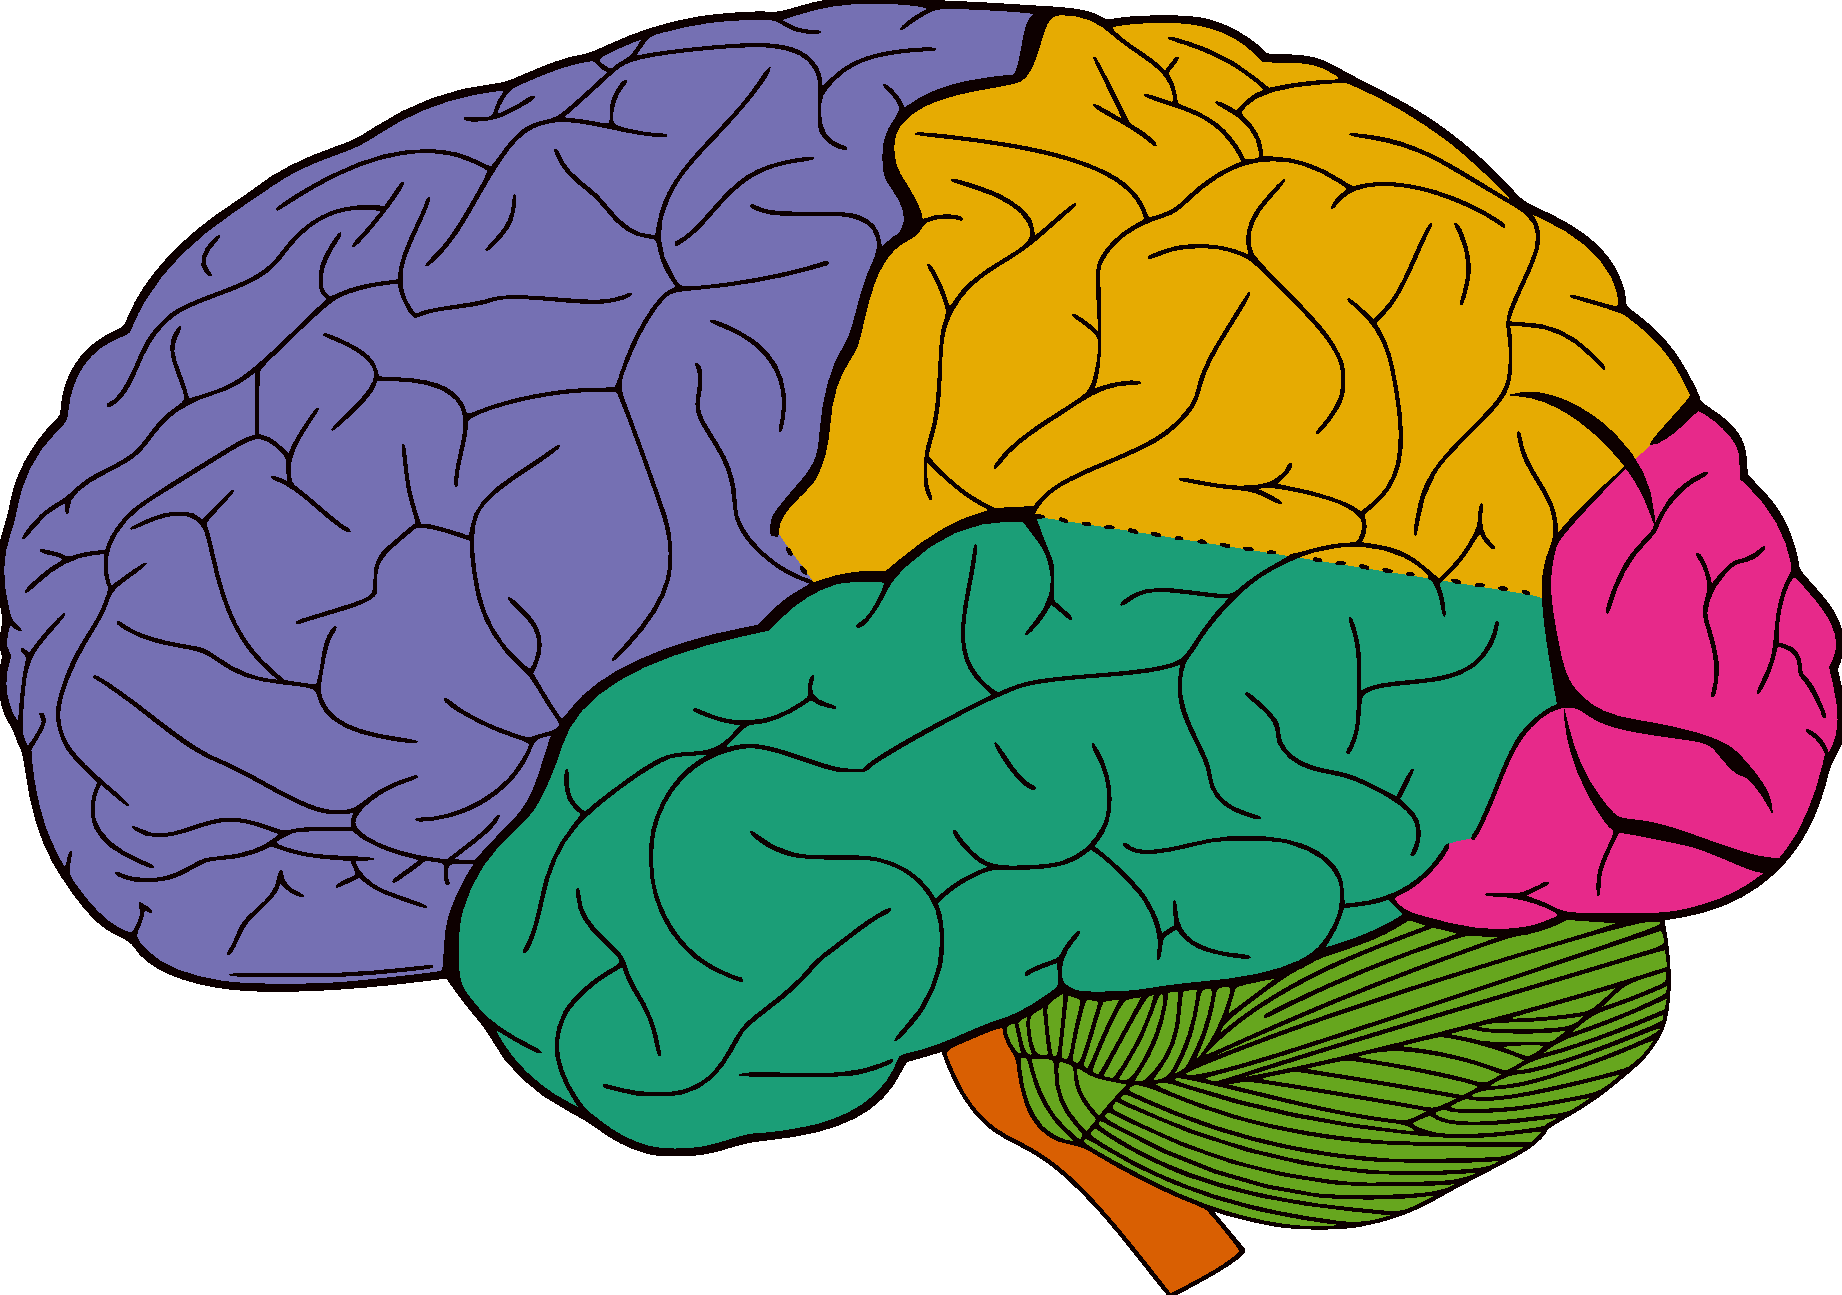
\includegraphics[height=3.25cm]{gfx/neuroanatomy/brain_lobes.pdf}}
\hspace*{\fill}
\subcaptionbox{\label{fig:nerveFiber}Origin: \url{https://en.wikipedia.org/wiki/Association_fiber}}[.47\textwidth]{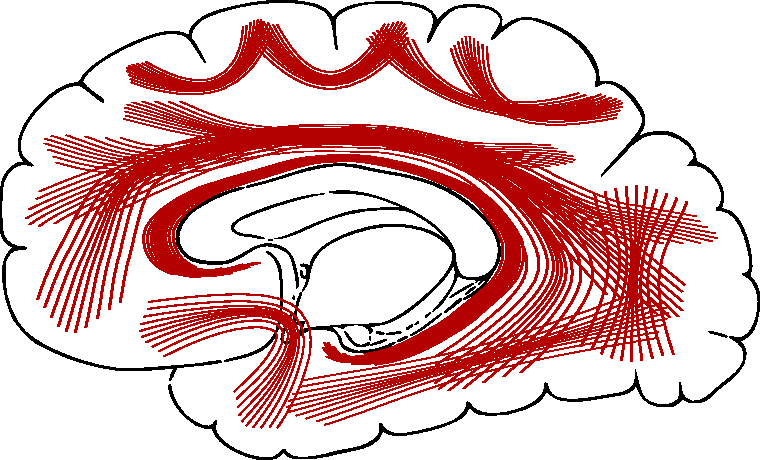
\includegraphics[height=3.25cm]{dev/wiki/brain_fiber_paths.png}}
% \hspace*{\fill}
\caption{(a) Illustration of human brain. (b) Illustration of a coronal human brain section. \todo{a) name brain parts, redo in inkscape}}
\label{fig:humanBrain}
\end{figure}
%
the frontal, parietal, temporal, and ocipital lobes (see \cref{fig:brainLobes}).
The frontal lobe contains the voluntary movements of specific body parts as well as the human personality.
The parietal lobe has \dummy{}.
The main function of the ocipital lobe is signal processing of the visual system.
The temporal lobes contain auditory functions and language in addition to visual memories.
\par
%
In the inner part of the brain there are also other structures such as the \dummy{}.
All these structures in the cerebellum and cerebrum contain along their surface a layer filled with cell bodies.
These cells have the task of processing the information of all signals coming from outside (and inside) the brain.
In addition, these cells are also arranged in other cortical layers that have different thicknesses, cell types, and densities depending on the brain area.
These cells have a relative high density and are not only locally interconnected with each other, but also with different brain areas (see \cref{fig:nerveFiber,fig:cortLayers}).
Therefore, the folding of the brain is particularly important to increase this layer and therefore the number of cells.
In the human brain there are several billions nerve cells.
There are many types of cells involved in this process, \eg{} granule or pyramidal cells.
Some cell types can amplify or inhibit a nerve signal.
This highly interconnected structure and arrangement of the various cells is the source of its high number of different functionalities and, in the case of the human being, the origin of its relative high intelligence and consciousness.
Therefore, it is a common goal of mankind to understand the human brain in order to improve both medical treatment and to understand the origin of intelligence in detail.
%
%
%
\section{Fiber architecture} \label{sec:fiberArchitecture}
%
\begin{figure}[!t]
\centering
% \hspace*{\fill}
\tikzset{external/export next=false}
\subcaptionbox{\label{fig:coronalStained}BB 4201: Gray, White Matter, Coronal Section, Stained}[0.64\textwidth]{
\begin{tikzpicture}[]
    \node[inner sep=0pt, anchor = south west] (fig) at (0,0)
    {\includegraphics[height=0.42\textwidth]{dev/brain/BB_4201.png}};
    \coordinate (WM1) at ($(fig.north west)!0.6!(fig.north east)$);
    \coordinate (WM2) at ($(fig.north east)!0.35!(fig.south east)$);
    \draw[RED, ultra thick, <-] (WM1 |- WM2) -- ++ (-42:0.75) node[pos=1, anchor=north] {\textbf{WM}};
    \coordinate (GM1) at ($(fig.north west)!0.275!(fig.north east)$);
    \coordinate (GM2) at ($(fig.north east)!0.125!(fig.south east)$);
    \draw[GREEN, ultra thick, <-] (GM1 |- GM2) -- ++ (-65:0.75) node[pos=1, anchor=north] {\textbf{GM}};
    % \draw (0,5) -- (10,5);
\end{tikzpicture}
}
\hspace*{\fill}
\subcaptionbox{Cortical layers\label{fig:cortLayers}}[0.34\textwidth]{
\includegraphics[height=0.42\textwidth]{dev/wiki/layers.png}
}
% \hspace*{\fill}
%
\caption[GM, WM, layers]{}
\label{fig:BBrain}
\end{figure}
%
%
%
\begin{figure}[!t]
\centering
% gfx/neuroanatomy/neuron-axon_.pdf
\begin{tikzpicture}[every node/.style={font=\small,},]
\node[anchor=south west] (F) at (0,0) {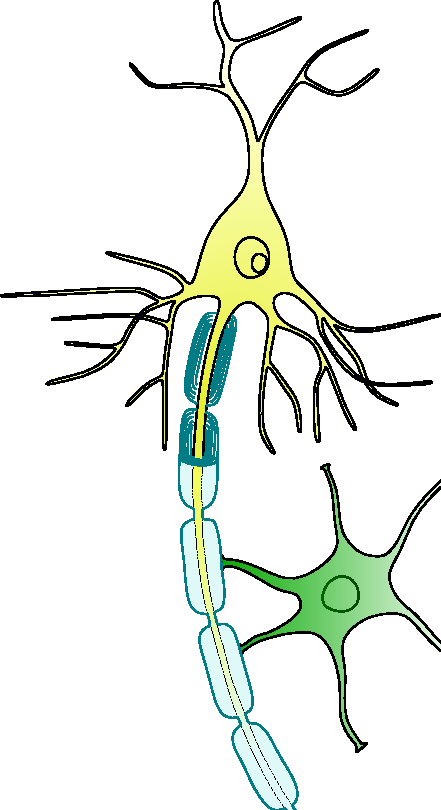
\includegraphics[angle=90,width=0.75\textwidth,]{gfx/neuroanatomy/neuron-axon.pdf}};
\begin{scope}[overlay]
    % \draw[] (0,0) grid (11,6);
    \node[] at (7.5,6.25) {Oligodendrocyte};
    \node[] at (2.5,1) {Cell Body};
    \node[anchor=west] at (10.5,3.9) {Axon};
    \node[] at (7.5,2.25) {Myelin};
    \draw[->] (2.75,2.75) -- (3.15,3.15) node[pos=0, anchor=north] {Nucleus};
    %
    \node[anchor=south] at (2.5,4.5) {Dendrites};
    \draw[->] (2.75,4.5) -- (3.5,4.25){};
    \draw[->] (2.25,4.5) -- (1.5,4.25){};
\end{scope}
\path[] ($(F.south west)-(1,0)$) -- ($(F.north east)+(1,0.6)$);
\end{tikzpicture}
\caption{
Illustration of a neuron with axon and oligodendrocytes. The olegodendrocyte build up a layered lipid structure up, surrounding the axon. The myelin layers are separated along the axon by nodes of Ranvier.}
\label{fig:human-brain}
\end{figure}
%
Nerve cells are connected by nerve fibers.
A typical nerve cell (see \cref{fig:human-brain}) (if there is such a thing) has a cell body, called a soma, that processes incoming information.
The information arrives via dendrites, which are star-shaped branches that connect to an incoming axon.
The axon is the only information output exit of the cell.
It travels through the brain to its destination, where it connects to with the axon terminal to a single or multiple locally brain cells .
\todo{in the case of human the development ...}
After the axons are formed in the brain, no new axons are formed.
Only the strength of the signals and the local structures change.
Among other things, connections that are not needed are also deleted during early development.
\par
%
Density of axons \dummy{}.
Its diameter ranges from about $\SI{0.5}{\micro\meter}$ to several $\si{\micro\meter}$ (see \cref{tag:axonDiameter}).
The axon is surrounded by a myelin layer, a lipid layer structure composed of nearby olegodendrides (see \cref{fig:human-brain}).
This environment electrically insulates the axon.
This improves the speed of propagation of the electrical action potential along the axon and also its signal strength.
There are many different types of axons.
Some contain a very thick myelin layer, while others have none.
The high density of axons and myelin makes the brain, where the axons are located, look white.
This is where this structure of the brain gets its name \ac{WM} from.
The outer cell body layer is called \ac{GM}.
This is even more visible in a Nissle stain, where the neurons absorb light (see \cref{fig:coronalStained}).
\par
%
%
% \begin{figure}[!t]
% 	\centering
% 	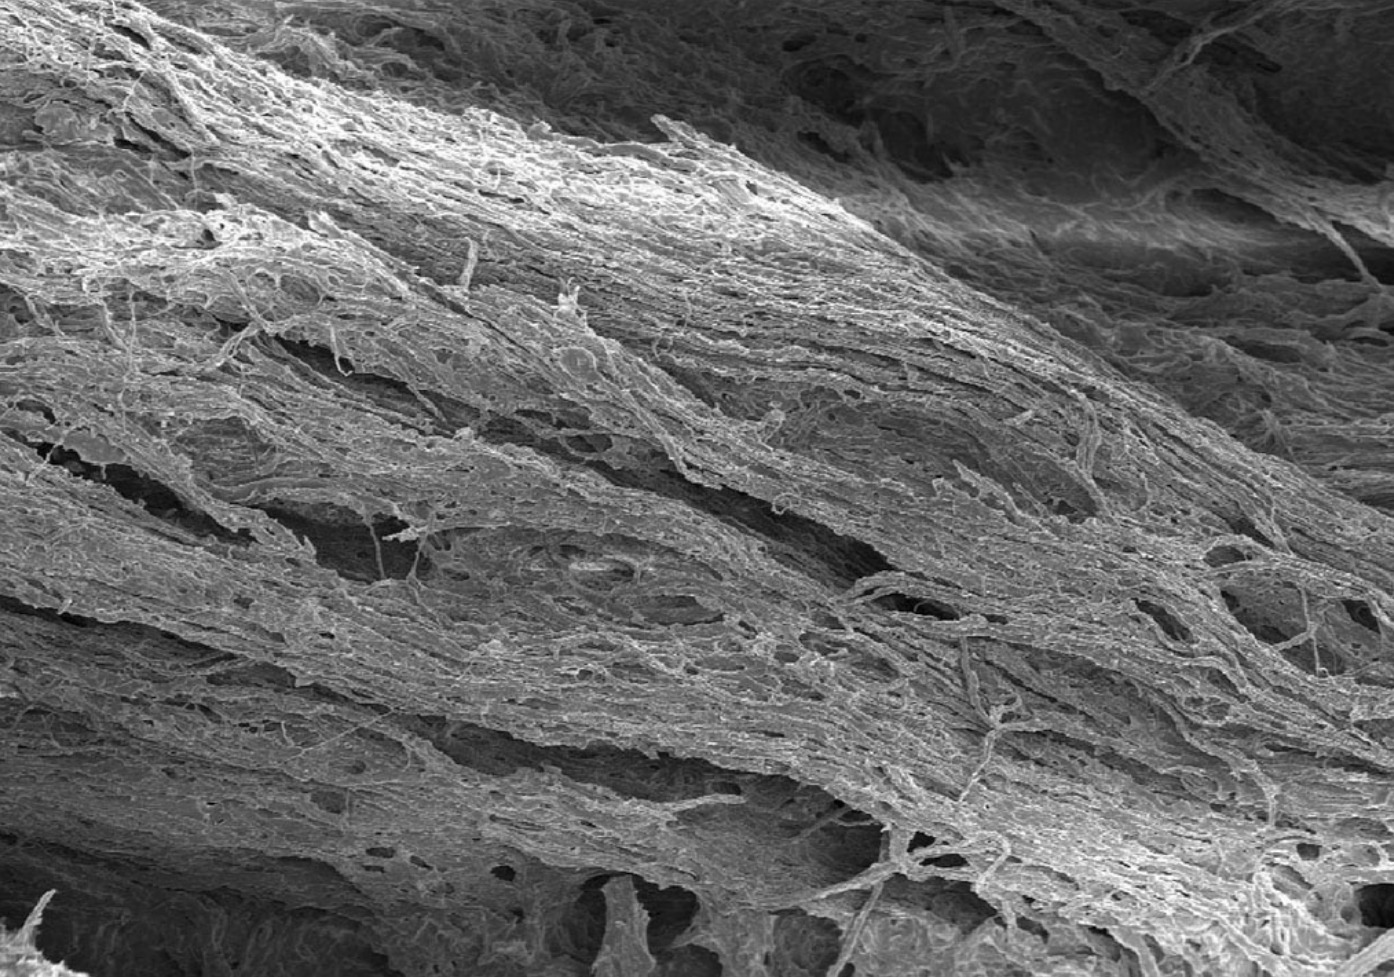
\includegraphics{gfx/neuroanatomy/human_wm_after_klinger_dissection.png}
% 	\caption{Electron microscopy image after klinger dissection \cite{destrieux:hal-01261930}. Fiber bundle structures are visible, following the same direction}
% % 	\label{fig:brain_sectioning}
% \end{figure}
%
\begin{figure}[!t]
	\centering
	\subcaptionbox{}[.49\textwidth]{
	    \includegraphics[width=0.45\textwidth]{dev/brain/auto_seg_axon_0.png}}\hfill
    \subcaptionbox{}[.49\textwidth]{
        \includegraphics[width=0.45\textwidth]{dev/brain/auto_seg_axon_1.png}}
	\caption{Automatic segmentet nerve fiber tissue from an electron microscopy \cite{Abdollahzadeh2019}. }
	\label{fig:elecMic}
\end{figure}
%
Because this \ac{WM} has such a high density of fibers, up to billions in the corpus calosum, which connects the left and right brain hemisphere, it is almost impossible, even under the microscope, to examine individual fiber tracts through the brain without additional aids.
One approach is myelin staining (see \cref{fig:brainMyelinStain}).
Here, nerve fibers that are myelinated absorb more light than their surroundings, resulting in high contrast.
Thus, even individual nerve fibers can be followed in section.
However, individual nerve fibers are already lost in smaller nerve fiber bundles.
Especially in dense white matter, information about the individual nerves can no longer be obtained.
It also has the disadvantage that no 3d orientation information can be easily determined.
\cref{fig:brainMyelinStain} shows a section using this technique in the human thalamus.
It shows different ways of organizing the nerve fibers.
Both nerve fiber bundles (orange) and network structures within the \ac{GM} are visible.
The latter are present to connect the nerve cells within the \ac{GM}, while the nerve fiber bundles allow the axons to reach their target area.
\par
%
\todo{klinger section}
%
\begin{figure}[!t]
	\centering
	\includegraphics{gfx/neuroanatomy/magic.png}
	\caption{Magic. TPFM auto fluorescence nerve fibers. Origin: \cite{Costantini2020}.}
	\label{fig:brainTPFM}
\end{figure}
%
\begin{figure}[!t]
	\centering
	\tikzset{external/export next=false}
	\begin{tikzpicture}[]  
        \node[inner sep=0pt, anchor = south west] (fig) at (0,0)
           {\includegraphics[width=\textwidth]{gfx/neuroanatomy/NeuralNet-BrainAtlasDotOrg.png}};
        %  
        \coordinate (A) at (fig.west);
        \coordinate (B) at (fig.west);
        %  
        \draw[Orange, ultra thick] (7.65,6.15) ellipse (1 and 0.5);
        \draw[ProcessBlue, ultra thick] (10,4.5) ellipse (2 and 1);
        \draw[white, ultra thick] ($(fig.south west)+(0.5,0.5)$) -- ++ (1.12697238cm,0) node[pos=0.5, above] {\small$\SI{100}{\micro\meter}$}; %13,87303cm/1231×(0,46×2)*...
        % \draw[yellow, ultra thick] (fig.north west) -- ++ (13.87303cm,0);
    \end{tikzpicture}
% 	\includegraphics[width=\textwidth]{gfx/neuroanatomy/NeuralNet-BrainAtlasDotOrg.png}
	\caption[Myelin staining of the human thalamus]{Myelin staining of the human thalamus, sagital section. \textcolor{Orange}{nerve fiber bundles}, \textcolor{ProcessBlue}{"neural net"}. \url{http://brainmaps.org/HBP3/h.sapiens/sag/h5thal-myelin/17a}}
	\label{fig:brainMyelinStain}
\end{figure}
%
Another technique is \ac{TPFM}.
\cref{fig:brainTPFM} shows a measurement after \ac{3D-PLI} using the \ac{MAGIC} protocol.
This allows fluorescence measurements of myelin. The fluorescence arises after the \ac{3D-PLI} sections are \cite{Costantini2021} washed with \ac{PBS}.
The figure shows the 3d structure of (species, region).
\ac{WM} is present in the lower left part of the volume.
The boundary between \ac{WM} and \ac{GM} is in the upper left to lower right figure.
In the upper right corner, \ac{GM} is present with both single nerve fibers and nerve fiber bundles.
\par
%
Another technique is electron microscopy (see \cref{fig:elecMic}).
It shows the tissue with a very high resolution, because the electrons have a much smaller wavelength.
The problem with this technique with tissue is that the measurement must take place in a vaccum, which allows the tissue to dry out.
This causes deformations.
Nevertheless, \cref{fig:elecMic} shows in high detail the layered structure that occurs in the white matter with nerve fibers of different myelin thickness.
\par
%
For different species with smaller brains, such as rodents, imaging techniques like \textit{clearing} [\dummy{}] have a high potential and could already be used to image a (whole?) brain with axons.
However, this has not yet been achieved for a more complex and larger brain.
Polarized light imaging (PLI), which uses the birefringence property of myelin, is a promising technique developed as early as 1900 that allows the orientation of axons to be mapped in a brain slice [\dummy{}].
This technique, like most microscopic techniques that use sections, has the disadvantage that the brain must be sectioned and then measured.
The cutting distorts the tissue and it must later be aligned in a nontrivial way to restore a complete brain dataset.
This process is also known as image registration.
There are alternative methods such as (OCT? \cite{Aumann2019}), which first measures the brain slice, then cuts away the top layer, and then measures the next slice. It uses the reflection of light rather than the light transmitted through the tissue.
However, no whole cerebrum such as a human brain has been measured in its entirety up to this point.
Since \ac{3D-PLI} uses the already known sectioning techniques that have been developed for several decades, it can use this knowledge to its advantage.
%
%
\section{Sectioning}
%
\begin{figure}[!t]
	\centering
    \setlength{\tikzwidth}{0.75\textwidth}
	\inputtikz{gfx/neuroanatomy/brain_sectioning}
	\caption{Illustration of sectioning. a)-b) block with imbedded brain, c) vibrating knife.}
	\label{fig:brain_sectioning}
\end{figure}
%
From Miriam thesis:
Brain removed from skull within \SI{24}{\hour} and immersed in a buffered solution of $\SI{4}{\percent}$ formaldehyde
$\SI{20}{\percent}$ glycerin solution for several days after \dummy{}.
$\SI{2}{\percent}$ Dimethyl sulfoxide (DMSO) and $\SI{4}{\percent}$ formaldehyde.
\par
% 
For the cutting process, the tissue, \ie{} the brain, has to be frozen and imbedded into a solid material.
One commen material is parafine, however this is not possible for \ac{3D-PLI} \todo{why?}.
For \ac{3D-PLI} it very is important, that the tissue does not build up crystal structures, \eg{} from sugar molecules, because these are also birefringence.
Therefore the tissue is first \dummy{} into a \dummy{} liquid \dummy{}
After a time of a few months the tissue will then be frozen into a $\SI{-80}{\degree}$.
Then the frozen tissue can be fixated with a liquid glue on a cutting plate.
The glue is \dummy{}
It is also be used to build up a surrounding fixating material to stabilize the brain in the cutting process.
Additionally markers are fixed which help in the later registration process, which will align the tissue sections in a 3d volume again \cite{Schober2016,Ali2018,Schmitz2018}.
\par
%
The cutting is done in a microtome (see \cref{fig:brain_sectioning}).
In there the temperature can be held at about $\SI{-70}{\degree}$ and allows no heating of the tissue.
The brain is moved against a vibrating very sharp knife.
This allows for the thin sectioning of about $\SI{60}{\micro\meter}$.
After the cutting, the tissue is put onto a glass specimen.
Since the tissue is such thin and filigran, it is not always possible to avoid cracks for example.
This also will be as best as possible corrected in the registration process.
The tissue will be \dummy{} with a glycerin \dummy{} and finally siled with another glass.
To prevent the formation of waves in the tissue, the glass is weighted.
The tissue sections are then stored into a refrigerator at $\SI{-70}{\degree\celsius}$.
The tissue can then finally be measured in the \ac{3D-PLI} microscopes (see \cref{sec:expSetup} for further techniqule informations).
%
%
\section{Axon Literature}
\label{sec:axonMicroscopy}
% 
\TODO{umschreiben}
%
Axon diameter \cite{Liewald2014}:
%
\begin{table}[!b]
\centering
\pgfplotstabletypeset[
thesisTableStyle,
font=\footnotesize,
col sep=comma,
columns/Name/.style={string type},
columns/Mean/.style={fixed zerofill},
columns/SD/.style={fixed zerofill},
columns/Median/.style={fixed zerofill},
columns/Max/.style={fixed zerofill},
columns/Min/.style={fixed zerofill},
columns/n/.style={dec sep align},
rowbf={1},rowbf={8},rowbf={19},
rowem={2},rowem={5},
rowem={9},rowem={12},rowem={15},
rowem={20},rowem={23},rowem={26},
]{data/axon_distribution.csv}
\caption{axon diameter distribution of the human brain in $\si{\micro\meter}$ \cite{Liewald2014}.}
\label{tag:axonDiameter}
\end{table}
%
\begin{table}[!b]
\centering
\pgfplotstabletypeset[
thesisTableStyle,
font=\footnotesize,
col sep=semicolon,
columns={article,cite,gratio},
columns/article/.style={string type, column name=name, column type = {l}},
columns/cite/.style={string type, column name=cite, column type = {l}},
columns/gratio/.style={string type, column name=$g_{\mathit{ratio}}$},
]{data/gratio.csv}
\caption{human $g_{\mathit{ratio}}$ from invivo mri studies.}
\label{tab:gratio}
\end{table}
%
axon = 0.5-1.0 diameter (most frequent
thickness of myelin mean = 0.09, median 0.08
-> g-ratio 0.9 (electron microscop, upper boundry)
%
g-ratio
\cite{Cercignani2017} -> 0.65-0.8 mrt, healty male and female different age, different regions\\
\cite{FitzGibbon2013} -> 0.58-0.84 (Retina), electron microscopy
%
\todo{brechungsindex}
%
% \begin{figure}[!t]
% 	\centering
% 	 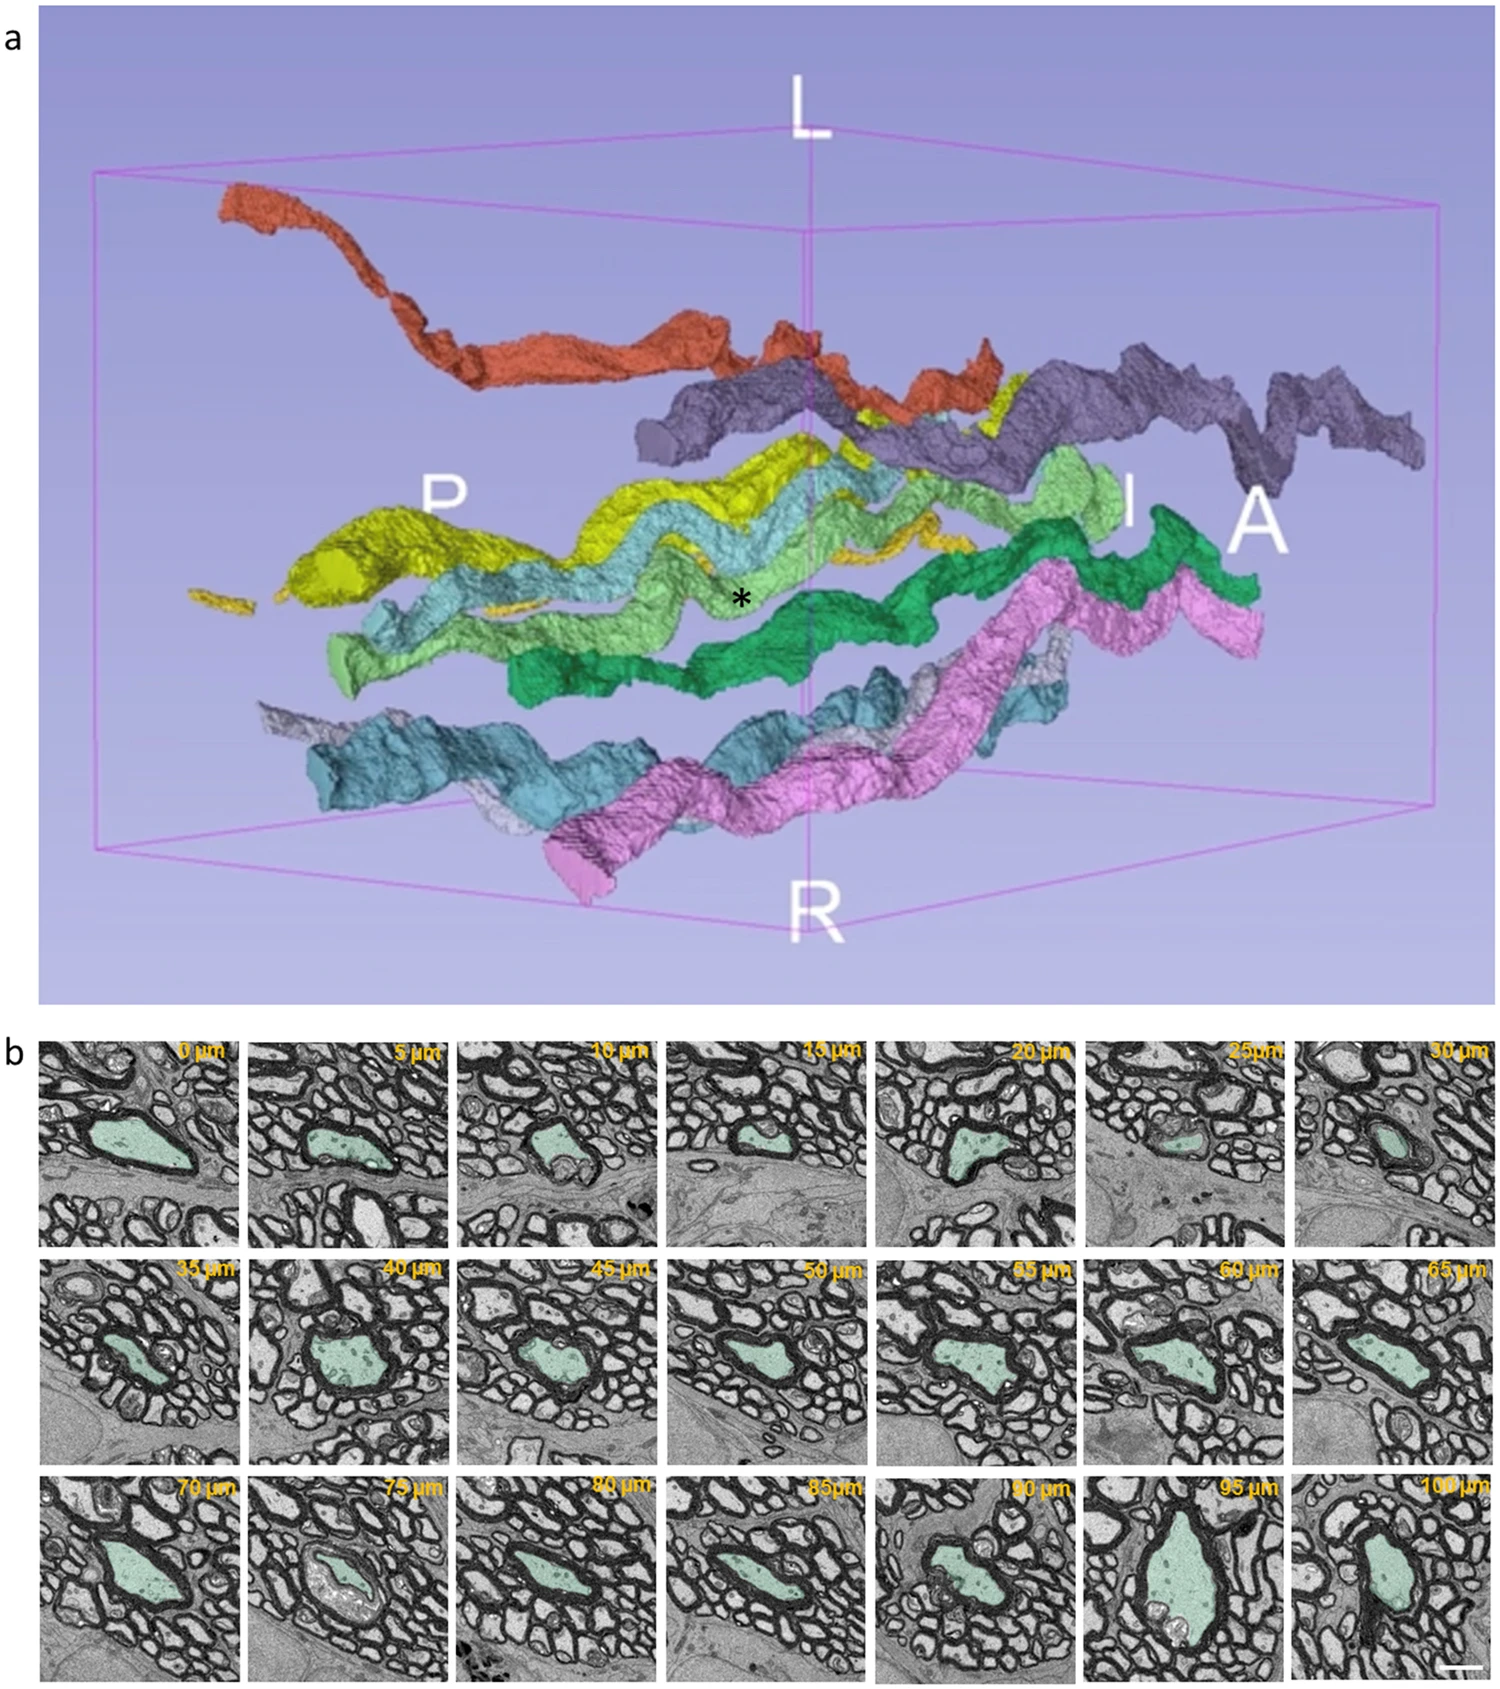
\includegraphics[clip, trim=0.65cm 6.25cm 0.4cm 0.5cm]{gfx/neuroanatomy/nature_3d_em_optical_nerve.png}
% 	\caption{\dummy{only show a} Three dimensional electron microscopy reveals changing axonal and myelin morphology along normal and partially injured (*, light green) optic nerves. Origin: \cite{Giacci2018} (reative Commons Attribution 4.0 International License).}
% % 	\label{fig:brain_sectioning}
% \end{figure}
%
%
% \par
% \noindent\rule{\textwidth}{2pt}
% \par
%